\newpage

\section{Deep Neural Network Monitor}
\label{sec6}

\subsection{Objectives and intuitions}

One of objectives of this project is to visualise, or ``monitor'' the CNN behaviour during the training phase. Thanks to the previous mentionned methods, users will have insights about the training phase and judge if the CNN has a strong or over-sized architecture and right parameters. Also, one might get visual indications on whether the training is running smoothly and the parameters converge to their correct values, or on the contrary whether training is ill-behaved and should re-initiated.
 
As we show in section \ref{sec2}, weights and gradients constitute key elements of deep neural networks. However, it is too complex to assess the quality of a CNN from brute values of weights and gradients at each epoch. It is therefore necessary to create custom metrics around gradients and weights to detect specific patterns like black areas, or highest and lowest activation areas of our network.

The custom metrics are the following :
\begin{itemize}
    \item loss and accuracy values for training and validation samples
    \item difference of weights between 2 consecutive epochs
    \item absolute value of gradients for one epoch
	\item activation map for each filter of the selected layer
	\item correlation between filters of the selected layer
\end{itemize}

The application developed in this section is largely based on the paper by \cite{Chen2018}. The latter proposes a number of visualisation techniques, in particular for the representation of weights, gradients, and activations along with their correlations. It is also the one paper demonstrated by the Ministry of Defense during their initial presentation, so the proposed visualisations were also part of the agenda for the project.

\subsection{Overview}


\subsubsection{Overall design}


Our application frontend comes as a dashboard (or graphical interface) composed of four quadrants:

\begin{enumerate}
	\item design of the network architecture
	\item loss and accuracy curves
	\item weights and gradiants visualization
	\item activation and correlation maps
\end{enumerate} 

The interface is fairly compact because we consider the tool as a POC \emph{(proof of conception)}. Developing a more user-friendly interface may constitute an improvement axis for further developments. For now, this framework proves suitable and convenient. 

\begin{figure}[H]
	\centering
	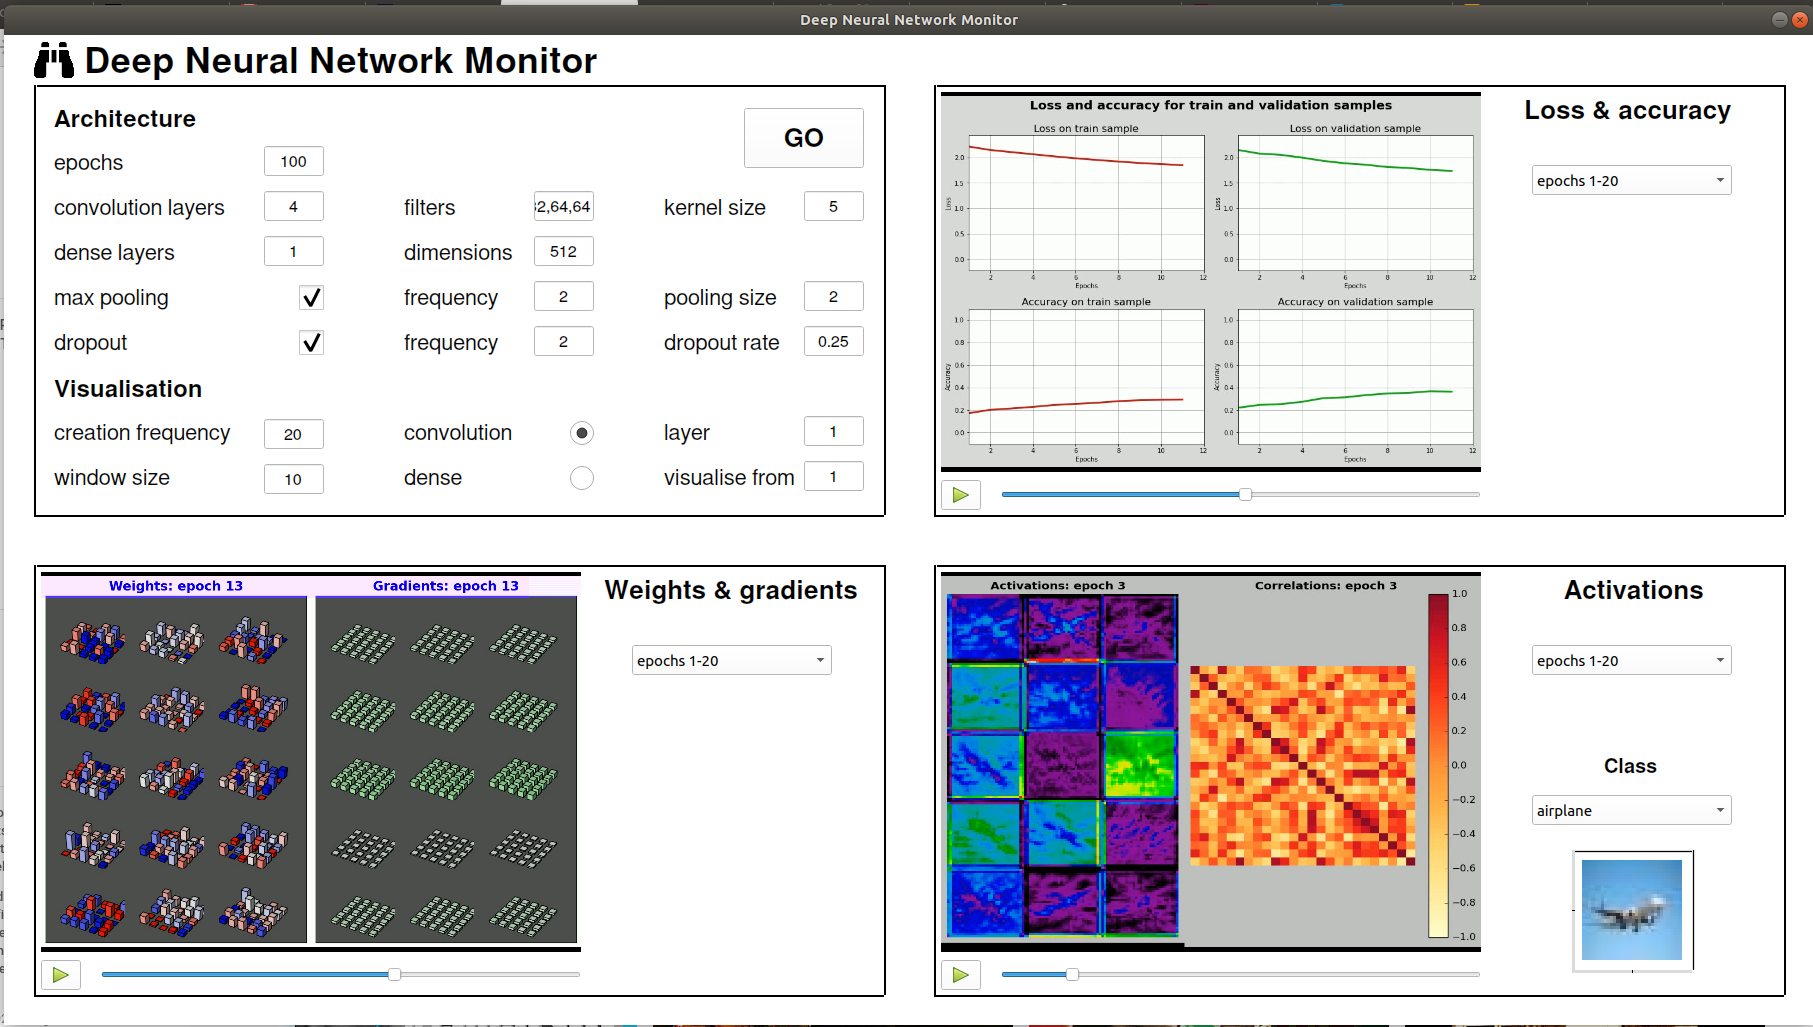
\includegraphics[scale=0.32]{images/weights-grads-viewer/frontend.png}
	\caption{Our application frontend}
\end{figure}

The backend consists in a set of modules with custom functions that need to be imported prior to starting the application. The python code then calls a Keras API which runs the designed CNN on the CIFAR 10 dataset. The information required for our visualizations is extracted by the way of callback functions and checkpoint processings, both included in tensorflow. Stream processing then provides visualisation in real time.

\begin{figure}[H]
    \centering
    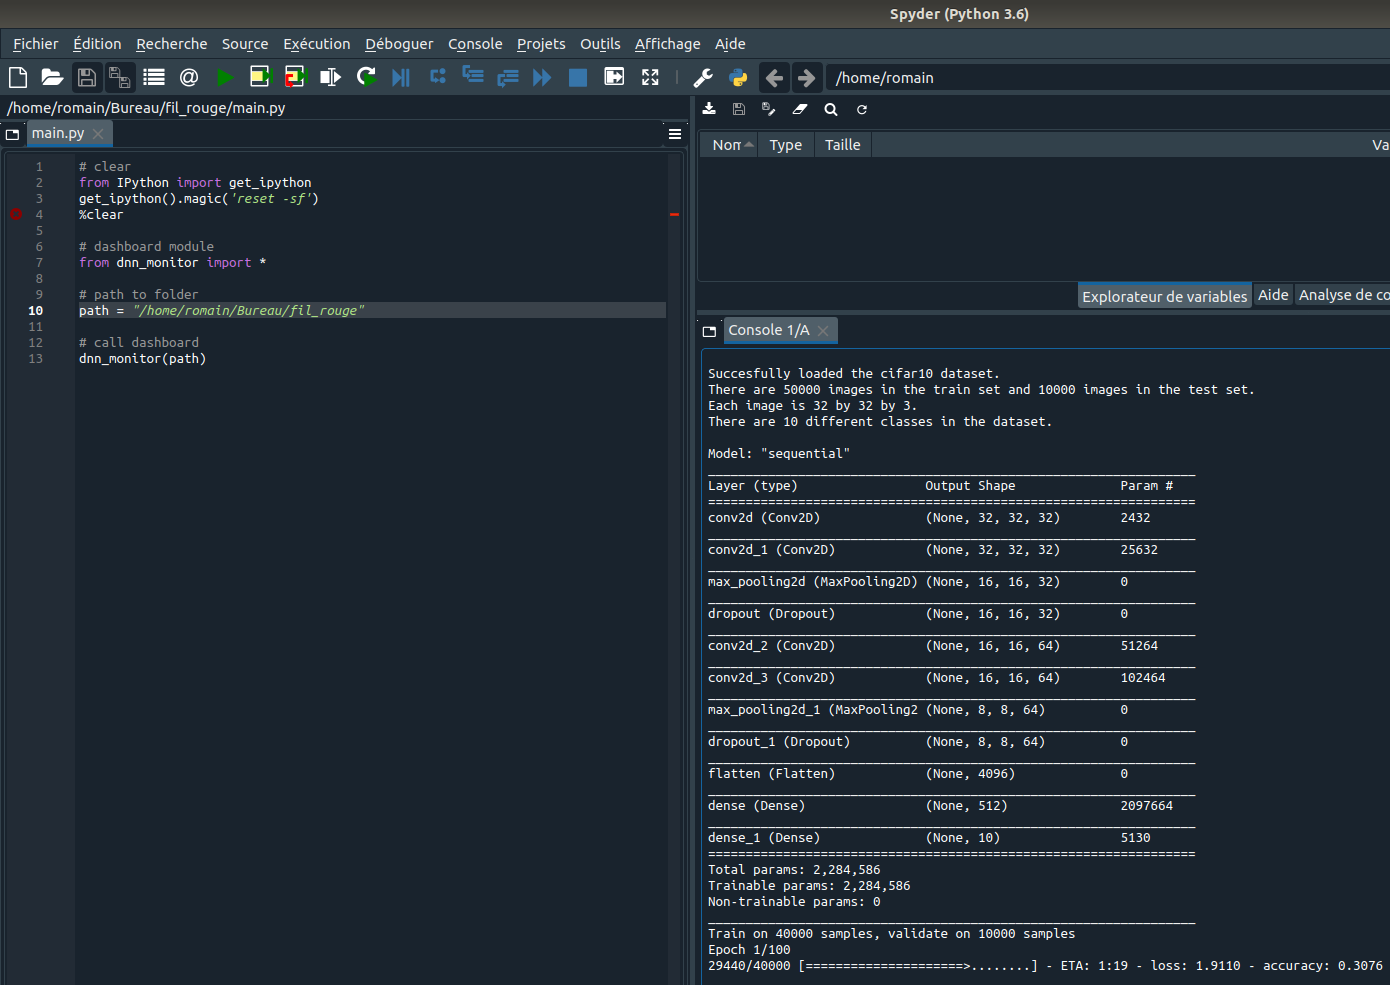
\includegraphics[scale=0.41]{images/weights-grads-viewer/backend.png}
    \caption{Backend: custom code and Keras API}
\end{figure}

\subsubsection{Model architecture}

The first step of our visualization device consists in determining the model architecture. The first quadrant of the dashboard is dedicated to this task and permits to set a number of options, offering some freedom in the design of the model. Among the options to be set are:

\begin{itemize}
    \item the number of convolution layers and the number of filters for each layer, along with the convolution kernel size
    \item the number of dense layers and their respective dimensions
    \item the use of max pooling and dropout with their frequencies and dimensions
\end{itemize} 

In terms of visualization, the lower part of the quadrant proposes to select:

\begin{itemize}
	\item the layer and neurons to be visualized
	\item the frequency at which the visualization must be updated in the dashboard
	\item the window size for the loss/accuracy plots of the second quadrant
\end{itemize} 

\begin{figure}[H]
    \centering
    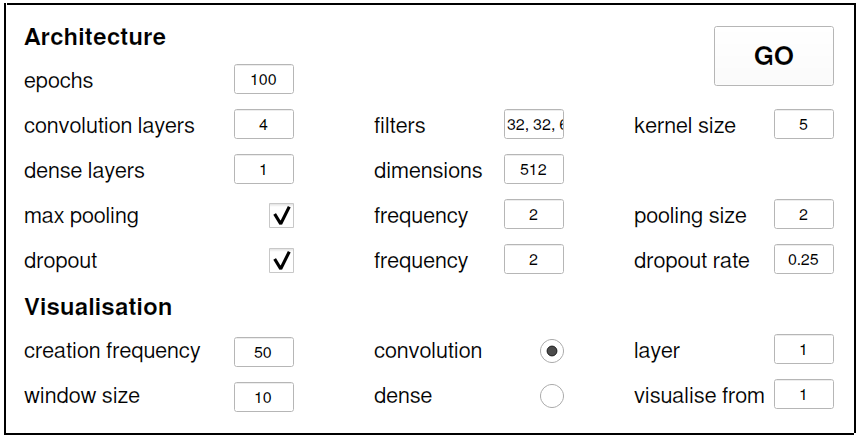
\includegraphics[scale=0.5]{images/weights-grads-viewer/Quadrant_architecture.png}
    \caption{We can customize our DNN thanks to the architecture quadrant}
\end{figure}


\subsection{Custom metrics}

\subsubsection{Accuracy and loss curves}

Accuracy and loss represent two basics metrics, but they are absolutly essential to follow the right or bad behavior of our network during training phase. Moreover, as is customary, we have split our reference dataset into two parts: train and validation. This provides a straightforward way to detect overfitting.   

\begin{figure}[H]
    \centering
    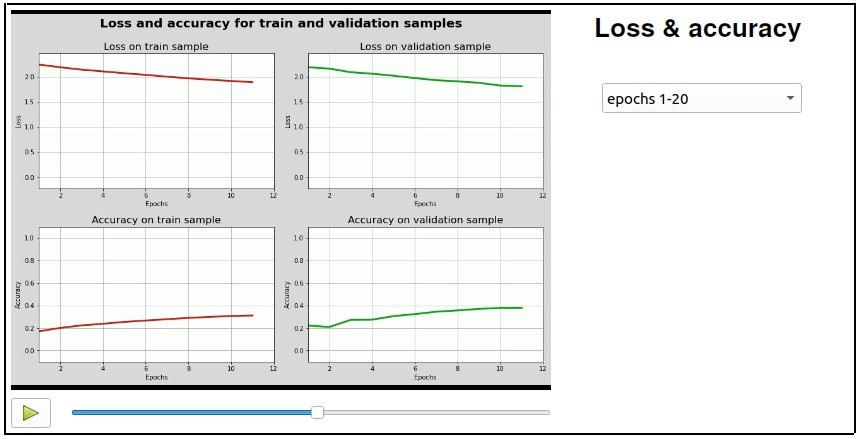
\includegraphics[scale=0.6]{images/weights-grads-viewer/Quadrant_loss.png}
    \caption{Evolution of loss and accuracy across epochs, for train and validation samples}
\end{figure}


\subsubsection{Gradients and Weights}

In this quadrant, we implemented a specific visualisation of weights and gradients evolution. In the panel, the left part is dedicated to weights while the right part represents the gradients. 

Regarding the weights:

\begin{itemize}
	\item red weights are positive, blue weights are negative
	\item the heights of the bars represent the weight value (in absolute value, after normalisation).
	\item the growth rate with respect to the previous period is represented by  color intensity. Pale weights evolve little, while intense color weights keep being updated.
	\item the weights are arganised by flattening filters over a row.
	\item a weight that never evolves and remains flat can be a ``dead'' weight that does not train properly
	\item a weight which keeps updating forever may indicate a difficulty of the model to converge to minimum of the loss function
\end{itemize} 

As for the gradients:

\begin{itemize}
	\item they are always displayed in green
	\item the size of the bars represents the (absolute and standardised) value of the gradient
	\item the color intensity is another proxy for the size, to help further distinguish strong from weak gradients
	\item a high gradient involves a weight still being updated (from back-propagation), a small gradient implies little update
\end{itemize}

\begin{figure}[H]
    \centering
    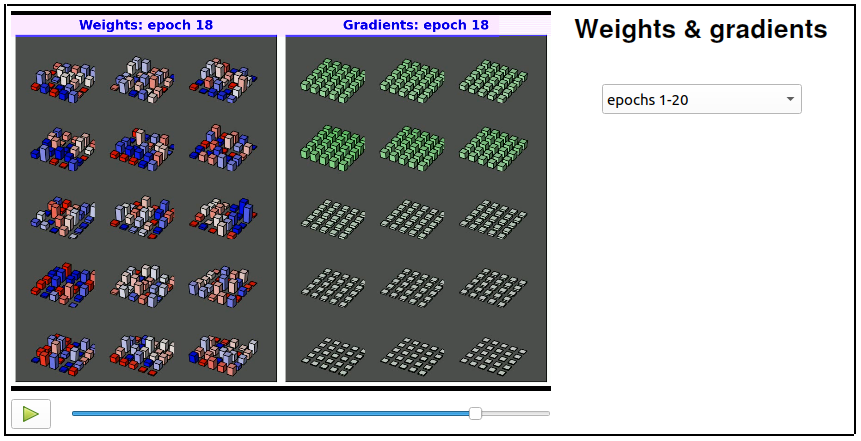
\includegraphics[scale=0.6]{images/weights-grads-viewer/Quadrant_weight.png}
    \caption{Evolution of gradients and loss for convolutional filters}
\end{figure}

\subsubsection{Activations and correlations}

The final metrics developped in the application consists in a display of the activation maps produced by the selected layer (on the left), and their correlations (on the right).

For activations:

\begin{itemize}
	\item each small square in the image represents the activation obtained from one filter of the layer
	\item the activation displayed is actually an average activation obtained over a batch of the class considered (small-sized: 10 images per batch)
	\item it is remarkable that even though the activations are obtained from a batch, they often produce recognizable images (like a ship on the example displayed below)
	\item an activation which remains dark is indicative of a ``dead'' filter which does not train properly
	\item two activations that look very similar may be a flag for redundant filters
\end{itemize}

Regarding correlations:

\begin{itemize}
	\item correlations are represented as a heatmap, where each square represents the correlation between two filters of the layer.
	\item the color code is a range from light yellow (strong negative correlation) to dark red (strong positive correlation)
	\item off-diagonal entries that are dark red imply a correlation close to 1 and thus suggest redundant filters
	\item off-diagonal entries that are light yellow imply a correlation close to -1 and may imply filters having similar but opposite effects
\end{itemize}


\begin{figure}[H]
	\centering
	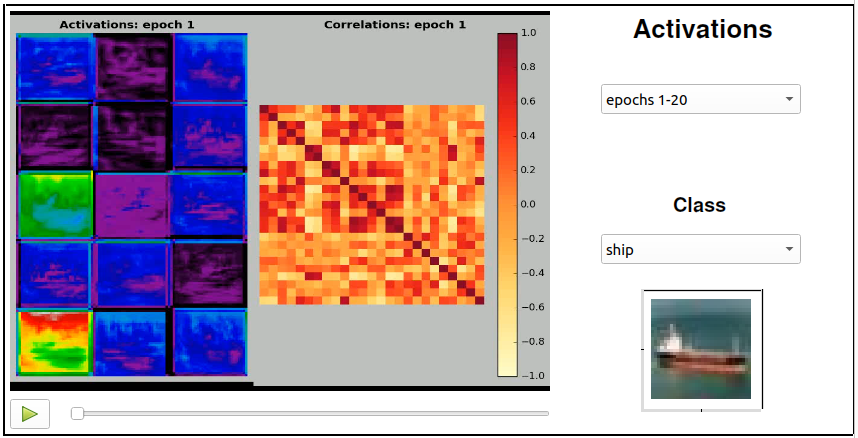
\includegraphics[scale=0.6]{images/weights-grads-viewer/Quadrant_activation.png}
	\caption{Evolution of activations and correlations for convolutional filters}
\end{figure}


\subsubsection{Conclusions on the DNN Monitor}

The DNN monitor provides a compact, intuitive and immediate view on a neural network across the different epochs of the training. One of its major assets is that it makes visualisation possible while training continues running in the background.

Individual views provided by the DNN Monitor can be useful, but it is really the conjugation of losses, accuracies, weights, gradients, activations, correlations and their evolution across training epochs which permits to obtain an overall assessment of the quality of the traning.









